Passing through the fog barrier, you stumble into a dream-like scene. The hallway is identical to the one in which you were previously interred, with one exception: large swathes of it are missing. You stand amongst a vast panorama of overcast sky and fog-choken environs. A few corpses lay in soft repose amongst the ruins.\\

A tile of flagstone breaks loose, dropping to the mezzanine below with a crack.\\

The man emerges from deeper within the ruins as if summoned by the sound. You finally get a look at his face, and find that it ignites something within your memories. He spoke the truth. This man played some major part in your life, though the details are lost to time.\\

"And now we will assess the salvage of our faithful."\\

The man turns his palms upwards, and a few of the corpses begin to stir.\\

"Prove yourself in service to the Black and Golden Key!"\\

\subsection*{Victory Condition}
Defeat Zealot Eóghainn

\subsection*{Setup Instructions}
\begin{center}
\framebox{
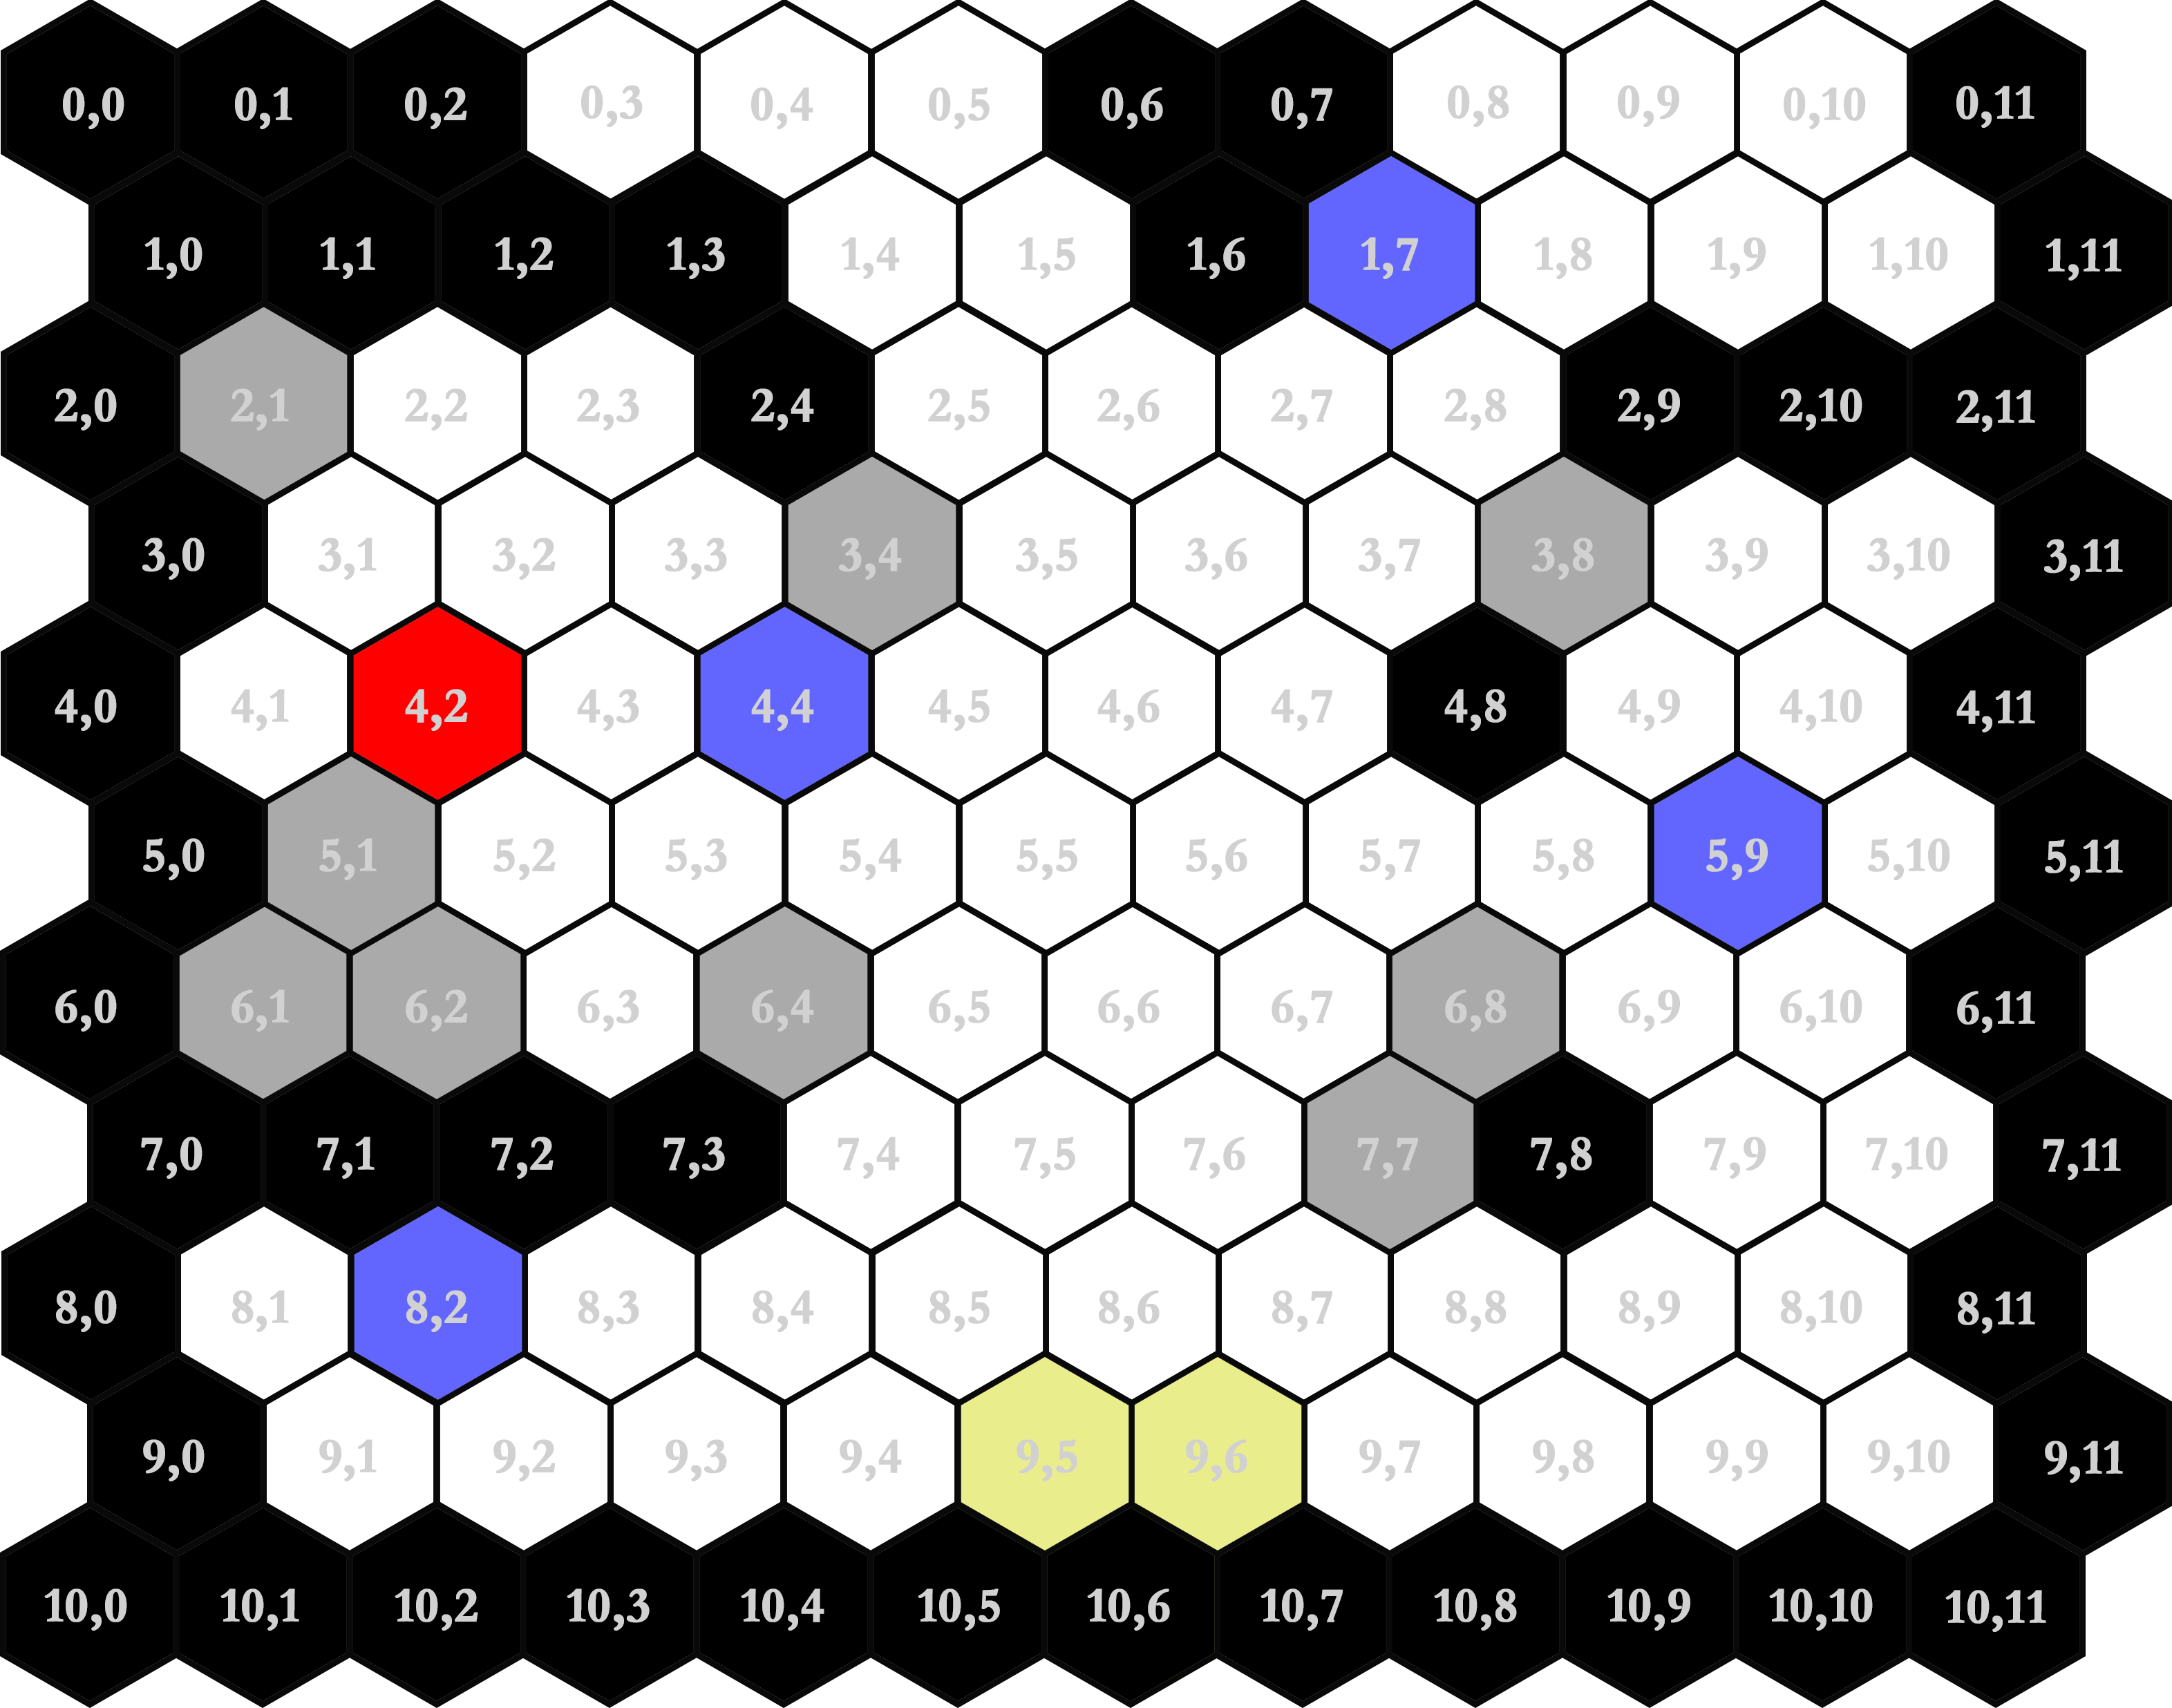
\includegraphics[width = 0.70\textwidth]{./maps/c317.png}
}
\end{center}

\subsection*{Setup Instructions}
\begin{itemize}
\item \textbf{Goldenrod:} Character Start Location. Place the character on either tile.
\item \textbf{Red:} Enemy Start Location. Place Zealot Eóghainn on this tile.
\item \textbf{Blue:} Enemy Start Location. Place a Risen Prisoner on \emph{two} of these tiles.
\item \textbf{Black:} Impassable Boundary/Full-Cover
\item \textbf{Light Gray:} Half-Cover.
\end{itemize}

\pagebreak

\begin{tcolorbox}
\subsection*{Doom Events}
\begin{itemize}
\item \textbf{Every 2nd Round:} \emph{Eóghainn steps into the fog.} Roll 2D6. Place Zealot Eóghainn on a hex located on either combination of the two dice scores. If neither location is valid, he remains in place.
\end{itemize}
\end{tcolorbox}

\subsection*{Encounter Table}
\begin{tcolorbox}
\textbf{Roll:} 1D6
\begin{center}
\begin{tabular}{ L | L | L }
\multicolumn{1}{c|}{\textbf{1}} & 
\multicolumn{1}{c|}{\textbf{2}} & 
\multicolumn{1}{c}{\textbf{3}} \\
\emph{Secret Parable} &
\textbf{A:} \emph{Secret Word}\newline \textbf{B:} \emph{Open-Palm Slap}\newline \textbf{C:} \emph{Secret Chant} &
\textbf{A:} \emph{Open-Palm Slap}\newline \textbf{B:} \emph{Secret Word} \\
\hline
\multicolumn{1}{c|}{\textbf{4}} & 
\multicolumn{1}{c|}{\textbf{5}} & 
\multicolumn{1}{c}{\textbf{6}} \\
\textbf{A:} \emph{Open-Palm Slap}\newline \textbf{B:} \emph{Secret Word} &
\textbf{A:} \emph{Secret Word}\newline \textbf{B:} \emph{Open-Palm Slap}\newline \textbf{C:} \emph{Secret Chant} &
\emph{Secret Parable} \\
\end{tabular}
\end{center}
\textbf{Note:} Each round, all Risen Prisoner enemies will Move towards the character and attempt \emph{Swipe}.
\end{tcolorbox}

\subsection*{Enemy Sheets}
\hrule
\ \\
{\large \textbf{Zealot Eóghainn}}\\\\
\begin{tabular}{s s s}
\textbf{HP:} 7 & \textbf{Move:} 2\\
\textbf{L.DEF}: 3 & \textbf{D.DEF:} 2\\
\end{tabular}\\

\emph{Intelligent:} This entity is human, or possesses a human-like intellect.\\

\textbf{Attacks:}
\begin{itemize}
\item \emph{Open-Palm Slap} -  Inflict Stun on an adjacent entity.
\item \emph{Secret Word} - Deal 1 \emph{Inevitable} Smite damage to an entity within 2-4 tiles.
\item \emph{Secret Chant} - Add 1 Enhanced Defense: \textbf{P.DEF} (1) condition token to this enemy sheet.
\item \emph{Secret Parable} - Roll 2D6. Place a Risen Prisoner on a hex located on either combination of the two dice scores. If neither location is valid, there is no effect.
\end{itemize}
\hrule
\ \\
{\large \textbf{Risen Prisoner}}\\\\
\begin{tabular}{s s s}
\textbf{HP:} 3 & \textbf{Move:} 4\\
\end{tabular}\\

\emph{Undead:} This entity ignores Bleed and Dark damage, and the Bleeding, Charmed, Maddened, and Fear conditions.\\

\textbf{Attack:}
\begin{itemize}
\item \emph{Swipe} -  Deal 1 \emph{Unparryable} Crush damage to an adjacent entity.
\end{itemize}
\pagebreak

\subsection*{Victory}
Eóghainn stumbles backwards a few steps, then drops to a knee and clutches his side.\\

“Very well.”\\

The man gasps and pants.\\
“You have... haa... passed the first of your trials. Haa... haa...”\\

He rakes a forearm across his brow, plastering the arm hairs against the skin, then stands.\\

“I am Eóghainn, of the Inner Circle.”\\

“And you say there are others? Doubtless they are in great want of guidance. ”\\

“Take me to them.”\\

\notegain{c317a} Zealot Eóghainn has been rescued\\
>> \turnto{c31}

\subsection*{Defeat}
You lay in defeat, a trio of risen prisoners shambling towards you with grasping hands. Then the man raises his arms, and they collapse in place.\\

“A valiant effort. But short nonetheless.”\\

The man approaches you with a hand outstretched, and lifts you onto your feet.\\

“I am Eóghainn, of the Inner Circle.”\\

“And you say there are others? Doubtless they are in great want of guidance. ”\\

“Take me to them.”\\

\notegain{c317a} Zealot Eóghainn has been... rescued\\
>> Clear all \textbf{HP} slots\\
>> \turnto{c31}